\documentclass[a4paper, 12pt]{article}
\usepackage{listings}
\usepackage[portuges]{babel}
\usepackage[utf8]{inputenc}
\usepackage{amsmath}
\usepackage{indentfirst}
\usepackage{graphicx}
\usepackage{multicol,lipsum}
\usepackage{float}
\usepackage[export]{adjustbox}
\usepackage{matlab-prettifier}

\usepackage{geometry}
 \geometry{
 a4paper,
 total={170mm,257mm},
 left=20mm,
 top=20mm,
 }

\begin{document}
%\maketitle

\begin{titlepage}
	\begin{center}
	
	%\begin{figure}[!ht]
	%\centering
	%\includegraphics[width=2cm]{c:/ufba.jpg}
	%\end{figure}

		\Huge{UTFPR}\\
		\large{Engenharia de Computação}\\ 
		\large{Controle Digital}\\ 
		\vspace{15pt}
        \vspace{95pt}
        \textbf{\LARGE{Projeto 3: Espaço de Estados }}\\
		%\title{{\large{Título}}}
		\vspace{3,5cm}
	\end{center}
	
	\begin{flushleft}
		\begin{tabbing}
			  Aluno: Deivid da Silva Galvão RA: 2408740\\
                Aluno: João Vitor Levorato De Souza
R.A: 2419890

\\
                Aluno: João Vitor N. Yoshida RA: 2419904\\
                Aluno: Thiago Berto Minson, RA: 2270412\\
			Professor orientador: Adalberto Zanatta Neder Lazarini \\
			%Professor co-orientador: \\
	\end{tabbing}
 \end{flushleft}
	\vspace{1cm}
	
	\begin{center}
		\vspace{\fill}
			 Fevereiro\\
		 2025
			\end{center}
\end{titlepage}
%%%%%%%%%%%%%%%%%%%%%%%%%%%%%%%%%%%%%%%%%%%%%%%%%%%%%%%%%%%

% % % % % % % % %FOLHA DE ROSTO % % % % % % % % % %

\begin{titlepage}
	\begin{center}
	
	%\begin{figure}[!ht]
	%\centering
	%\includegraphics[width=2cm]{c:/ufba.jpg}
	%\end{figure}

		\Huge{UTFPR}\\
		\large{Engenharia de Computação}\\ 
		\large{Controle Digital}\\ 
\vspace{15pt}
        
        \vspace{85pt}
        
		\textbf{\LARGE{Projeto 3: Espaço de Estados}}
		\title{\large{Título}}
	%	\large{Modelo\\
     %   		Validação do modelo clássico}
			
	\end{center}
\vspace{1,5cm}
	
	\begin{flushright}

   \begin{list}{}{
      \setlength{\leftmargin}{4.5cm}
      \setlength{\rightmargin}{0cm}
      \setlength{\labelwidth}{0pt}
      \setlength{\labelsep}{\leftmargin}}

      \item Relatório do Trabalho Prático Disciplinar apresentado como requisito parcial à obtenção de nota na disciplina de Controle Digital do Curso Superior de Engenharia de Computação da Universidade Tecnológica Federal do Paraná.

      \begin{list}{}{
      \setlength{\leftmargin}{0cm}
      \setlength{\rightmargin}{0cm}
      \setlength{\labelwidth}{0pt}
      \setlength{\labelsep}{\leftmargin}}

                \item Aluno: Deivid da Silva Galvão RA: 2408740\\
               \item  Aluno: João Vitor Levorato De Souza
R.A: 2419890\\
                \item Aluno: João Vitor N. Yoshida RA: 2419904\\
                \item Aluno: Thiago Berto Minson, RA: 2270412\\
            \item Professor orientador:  Adalberto Zanatta Neder Lazarini \
      		%\item Professor co-orientador: \

      \end{list}
   \end{list}
\end{flushright}
\vspace{1cm}
\begin{center}
		\vspace{\fill}
		 Fevereiro\\
		 2025
			\end{center}
\end{titlepage}
\newpage
% % % % % % % % % % % % % % % % % % % % % % % % % %
\newpage
\tableofcontents
\thispagestyle{empty}

\newpage
\pagenumbering{arabic}
% % % % % % % % % % % % % % % % % % % % % % % % % % %
\section{Introdução}
    No projeto 3, vamos aplicar os conceitos aprendidos anteriormente para modelar um sistema de controle para um motor de corrente contínua utilizando a teoria de espaço de estados. O sistema será representado pelo seguinte esquema:

\begin{figure}[H]
    \centering
    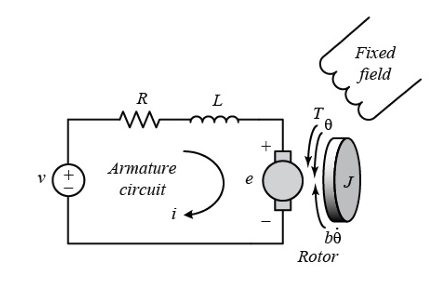
\includegraphics[width=0.6\linewidth]{sis.png}
    \caption{Esquemático do Motro CC}
    \label{fig:enter-label}
\end{figure}
    Descrito pelo modelo de espaço de estados da Equação:
    \begin{equation}
     x(t)=\begin{bmatrix}
            - \frac{b}{J} & \frac{Kt}{J} \\
                - \frac{Kg}{L} & - \frac{Ra}{L} 
    \end{bmatrix} =
    \begin{bmatrix}
            \(\omega\)(t) \\
            ia(t) 
    \end{bmatrix}
    +
    \begin{bmatrix}
            0 \\
            \frac{1}{La} 
    \end{bmatrix}
    u(t)  
    \end{equation}
sendo 

\begin{itemize}
    \item \textbf{Ra}: Resistência da armadura
    \item \textbf{La}: Indutância da armadura
    \item \textbf{Kt}: Constante de torque do motor
    \item \textbf{Kg}: Constante de força contra-eletromotriz
    \item \textbf{b}: Coeficiente de atrito viscoso
    \item \textbf{J}: Momento de inércia do motor
    \item \textbf{ia} Corrente de armadura
    \item \textbf{\(\omega\)}: Velocidade do motor
\end

Para este projeto, utilizaremos os seguintes valores
J = 0,2 kg·m², b = 0,7 N·m·s, Kg = 0,4 V/(rad/s), Kt = 0,1 N·m/A, Ra = 10Ω, La = 1H
\newpage
\section{Implementação}


\subsection{Verificação de Controlabilidade}
    Um sistema dinâmico de espaço de estados é composto por quatro matrizes ou vetores principais. No âmbito deste projeto, temos a matriz de parâmetros do sistema "A", que está relacionada com o vetor de estados. Os outros três vetores de parâmetros do sistema são "B", "C" e "D". O vetor "B" está relacionado com o sinal de entrada, o vetor "C" com o vetor de estados no sinal de saída e o vetor "D" com o sinal de entrada no sinal de saída.
    
    Dessa forma, as equações assumem o seguinte formato:
    \[
    \dot{x}(t) = A x(t) + B u(t)
    \]
    
    \[
    y(t) = C x(t) + D u(t)
    \]

    As matrizes \( A \) e \( B \) são definidas pelo modelo de espaço de estados do sistema controlado. A matriz \( C \) especifica a saída de interesse, enquanto \( D \) é zero, pois a alimentação direta não se aplica ao projeto. Substituindo os valores nas matrizes, temos:

    \[
    A = \begin{bmatrix}
    -\frac{b}{J} & \frac{K_t}{J} \\
    -\frac{K_g}{L} & -\frac{R_a}{L}
    \end{bmatrix} = \begin{bmatrix}
    -\frac{0,7}{0,2} & \frac{0,1}{0,2} \\
    -\frac{0,4}{1} & -\frac{10}{1}
    \end{bmatrix} = \begin{bmatrix}
    -3,5 & 0,5 \\
    -0,4 & -10
    \end{bmatrix}
    \]
    
    \[
    B = \begin{bmatrix}
    0 \\
    \frac{1}{L}
    \end{bmatrix} = \begin{bmatrix}
    0 \\
    \frac{1}{1}
    \end{bmatrix} = \begin{bmatrix}
    0 \\
    1
    \end{bmatrix}
    \]
        
    \[
    C = \begin{bmatrix}
    1 & 0
    \end{bmatrix}
    \]
     
    \[
    D = 0
    \]


    Antes de definir os sistemas de controle, é preciso verificar a controlabilidade do sistema. No Matlab, isso é feito com o comando "\textit{ctrb}", que recebe as matrizes \( A \) e \( B \) e retorna a matriz de controlabilidade, mostrada a seguir:

    \[
    \text{ctrb}(A,B) = \begin{bmatrix}
    0 & 0.5 \\
    1 & -10
    \end{bmatrix}
    \]

    Para verificar a controlabilidade do sistema, é necessário avaliar se a matriz de controlabilidade é invertível. Isso é feito calculando seu determinante: se for zero, a matriz não é invertível e o sistema não é controlável. Assim, ao calcular o determinante da matriz de controlabilidade do sistema em análise, obtemos:
    \[
    \text{det}(\text{ctrb}(A,B)) = \text{det} \begin{bmatrix}
    0 & 0.5 \\
    1 & -10
    \end{bmatrix} = (0 * (-10)) - (0.5 * 1) = -0.5
    \]
    Como o determinante resultou em -0.5, pode-se concluir que a matriz pode ser invertível e portanto o sistema pode ser controlado.

\subsection{Parte 1: Controle por regulação}
    Inicialmente, foi feito o \textit{plot} da resposta do sistema a uma entrada degrau e impulso, com o intuito de ter uma compreensão inicial do comportamento do sistema  A seguir, são apresentados os gráficos correspondentes, nas Figuras 2 e 3.


    \begin{figure}[H]
        \centering
        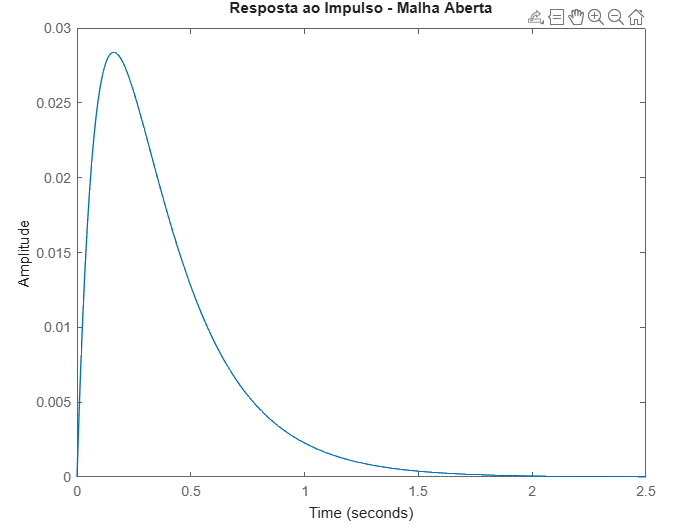
\includegraphics[width=0.75\linewidth]{impulse.png}
        \caption{Resposta ao Impulso}
        \label{fig:enter-label}
    \end{figure}

    \begin{figure}[H]
        \centering
        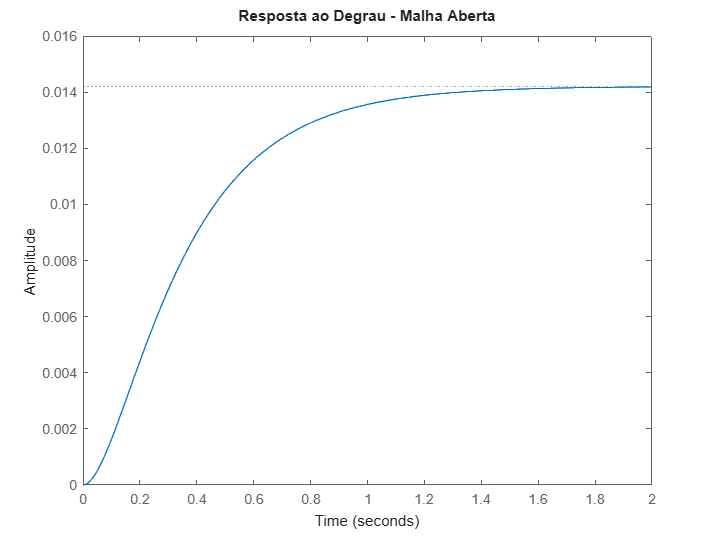
\includegraphics[width=0.75\linewidth]{step.png}
        \caption{Resposta ao Degrau}
        \label{fig:enter-label}
    \end{figure}

   As respostas para ambas as entradas não são as esperadas. Na entrada degrau, o valor final é baixo, assim como o valor máximo na entrada impulso, ambos na ordem de \( 10^{-2} \). Isso indica a necessidade de regulação para melhorar as respostas. Para isso, utiliza-se a função `place` do Matlab, que recebe as matrizes \( A \) e \( B \) e dois polos (um para cada estado). Os polos escolhidos foram -5 e -6.
   Atendendo aos requisitos do projeto, o sistema é simulado para condições iniciais \([105 \ 0]\) e uma entrada degrau unitário com valor final 105. As simulações mostram que, para diferentes ganhos, o comportamento do sistema varia significativamente, possivelmente devido à influência dos polos nos ganhos e no erro de regime permanente. A seguir, são apresentadas as respostas do sistema com condições iniciais \([105 \ 0]\) para uma entrada degrau unitário (Figuras 4 e 5).
   \begin{figure}[H]
       \centering
       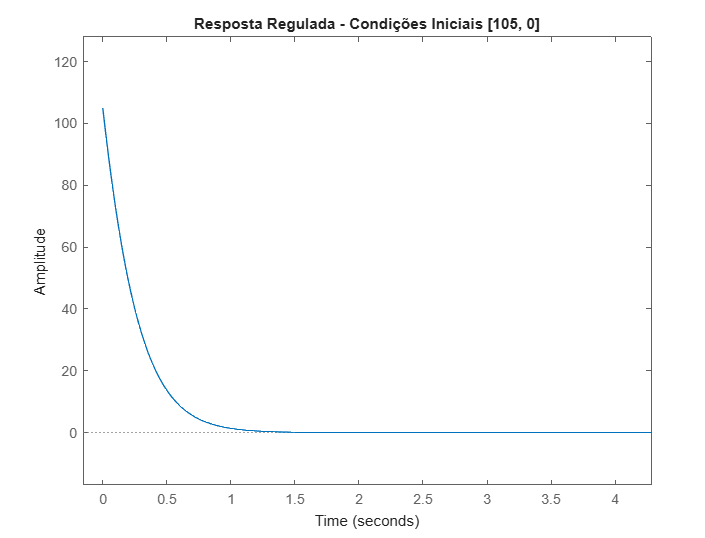
\includegraphics[width=0.75\linewidth]{Step2.png}
       \caption{Condições iniciais}
       \label{fig:enter-label}
   \end{figure}
   
   \begin{figure}[H]
       \centering
       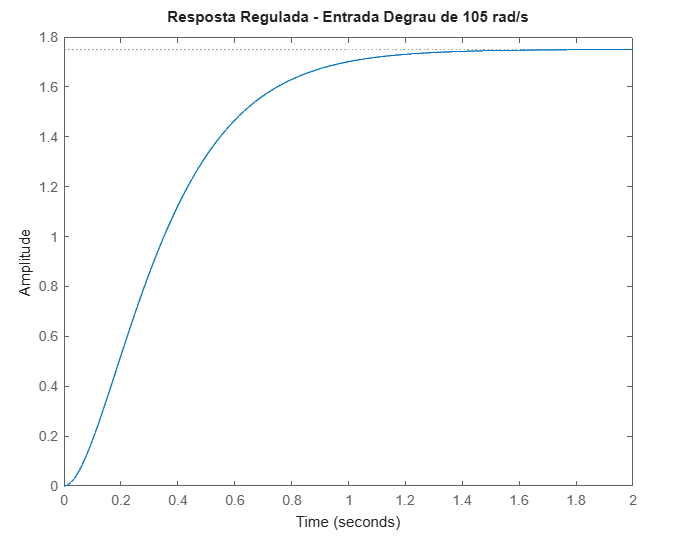
\includegraphics[width=0.75\linewidth]{stepcontrl.png}
       \caption{entrada degrau unitário de valor final 105}
       \label{fig:enter-label}
   \end{figure}

\subsection{Parte 2: Controle por rastreio}
    Analisando as respostas do sistema regulado, percebe-se que o erro em regime permanente é predominante. Para corrigi-lo, utiliza-se um integrador, cuja função é eliminá-lo. Esse integrador recebe um ganho \( h \) e é alimentado pela diferença entre a entrada e a saída do sistema. Após a integração, o resultado é ajustado pela realimentação dos ganhos. Para calcular os ganhos \( k_1 \), \( k_2 \) e \( h \), considera-se a seguinte matriz:
    
    \[
    P = \begin{bmatrix}
    A - B k & B h \\
    -C & 0
    \end{bmatrix}
    \]

    Os autovalores são calculados, resultando em três equações que são igualadas a três polos escolhidos. A resolução desse sistema fornece os valores dos ganhos \( k_1 \), \( k_2 \) e \( h \). 
    
    Os polos selecionados (\(-10\), \(-15\) e \(-20\)) garantem uma resposta rápida, atendendo aos requisitos do projeto (tempo de estabelecimento menor que 0.8s e sem *overshoot*). A seguir, são apresentadas as respostas do sistema para uma entrada degrau com valor final 105 rad/s (Figura 6) e para uma entrada de onda quadrada (Figura 7), permitindo comparação com o sistema regulado.
    

\begin{figure}[H]
    \centering
    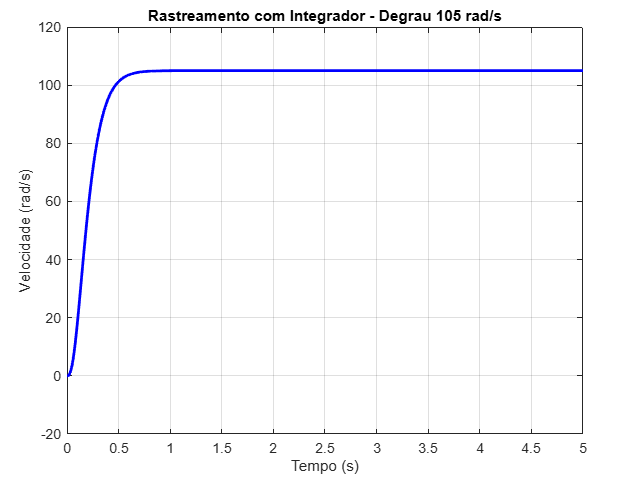
\includegraphics[width=0.75\linewidth]{stepRastreio.png}
    \caption{Resposta Entrada Degrau de 105 rad/s}
    \label{fig:enter-label}
\end{figure}

\begin{figure}[H]
    \centering
    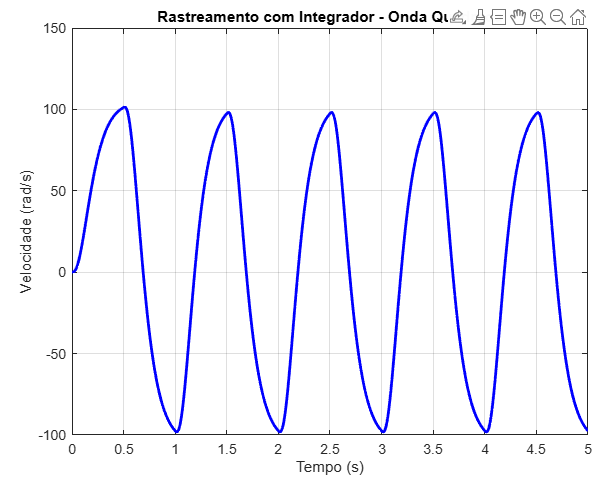
\includegraphics[width=0.75\linewidth]{SenoideRastreio.png}
    \caption{Resposta Entrada Senoidal (Onda Quadrada)}
    \label{fig:enter-label}
\end{figure}
   
\subsection{Código Matlab}

\begin{lstlisting}[
frame=single,
numbers=left,
style=Matlab-Pyglike]
Alunos:
Deivid da Silva Galvao RA: 2408740
Joao Vitor Levorato De Souza R.A: 2419890
Joao Vitor N. Yoshida RA: 2419904
Thiago Berto Minson, RA: 2270412
%% Projeto Controle Digital - Espaco de Estados
% Resolucao completa do projeto fornecido

%% 1. Definicao das matrizes do sistema
J = 0.2;   % Momento de inercia (kg.m^2)
b = 0.7;   % Coeficiente de atrito viscoso (N.m.s)
Kg = 0.4;  % Constante de forca contra-eletromotriz (V/rad/s)
Kt = 0.1;  % Constante de torque do motor (N.m/A)
Ra = 10;   % Resistencia da armadura (Ohm)
L = 1;     % Indutancia da armadura (H)

A = [-b/J Kt/J; -Kg/L -Ra/L]
B = [0; 1/L]
C = [1 0];
D = 0;

%% 2. Verificacao da controlabilidade
Co = ctrb(A, B)
determinante_Co = det(Co)
controlavel = rank(Co) == size(A,1);

%% 3. Resposta em malha aberta
sys_open = ss(A, B, C, D);
figure;
impulse(sys_open);
title('Resposta ao Impulso - Malha Aberta');
figure;
step(sys_open);
title('Resposta ao Degrau - Malha Aberta');

%% 4. Controlador por Regulacao
p_reg = [-5 -6]; % Polos escolhidos
K_reg = place(A, B, p_reg);
A_cl_reg = A - B*K_reg;
sys_cl_reg = ss(A_cl_reg, B, C, D);

% Resposta para condicoes iniciais [105 0]
figure;
initial(sys_cl_reg, [105; 0]);
title('Resposta Regulada - Condicoes Iniciais [105, 0]');

% Resposta para entrada degrau de 105 rad/s
figure;
step(105 * sys_cl_reg);
title('Resposta Regulada - Entrada Degrau de 105 rad/s');

%% 5. Controlador por Rastreamento
% Especificacao para alocacao de polos:
% Para um tempo de estabelecimento menor que 0,8 s e sem overshoo
% Sistema aumentado
A_aug = [A,zeros(2,1);
         -C,0 ];

B_aug_u = [B; 0];        
B_aug_r = [0; 0; 1];  

C_aug = [C, 0];   
D_aug = 0;

% Verifique a controlabilidade com respeito a B_aug_u
Co_aug = ctrb(A_aug, B_aug_u);
disp(['Posto da controlabilidade (A_aug,B_aug_u) = ', num2str(rank(Co_aug))]);

%% Escolha dos polos desejados
% Para rastreamento sem overshoot e tempo de estabelecimento < 0,8s,

p_desired_aug = [-10, -15, -20];

%% Calcular o vetor de ganhos [K, kI]
K_aug = place(A_aug, B_aug_u, p_desired_aug);
K = K_aug(1:2);
kI = K_aug(3);

disp('Ganhos encontrados:');
disp(['K = [', num2str(K), '], kI = ', num2str(kI)]);

%% Montar o sistema em malha fechada (com integrador)
A_cl = A_aug - B_aug_u * K_aug; 
B_cl = B_aug_r;                  
C_cl = C_aug;
D_cl = 0;

sys_cl = ss(A_cl, B_cl, C_cl, D_cl);

%% Simulacao - Degrau de 105 rad/s
t = 0:0.01:5;
r = 105 * ones(size(t));

[y, ~, ~] = lsim(sys_cl, r, t);

figure;
plot(t, y, 'b', 'LineWidth', 2);
xlabel('Tempo (s)');
ylabel('Velocidade (rad/s)');
title('Rastreamento com Integrador - Degrau 105 rad/s');
grid on;

%% Simulaaco - Onda quadrada
r_sq = 105 * square(2*pi*1*t);  % 1 Hz
[y_sq, ~, ~] = lsim(sys_cl, r_sq, t);

figure;
plot(t, y_sq, 'b', 'LineWidth', 2);
xlabel('Tempo (s)');
ylabel('Velocidade (rad/s)');
title('Rastreamento com Integrador - Onda Quadrada');
grid on;
\end{lstlisting}

\subsection{Simulink}

\begin{figure}[H]
    \centering
    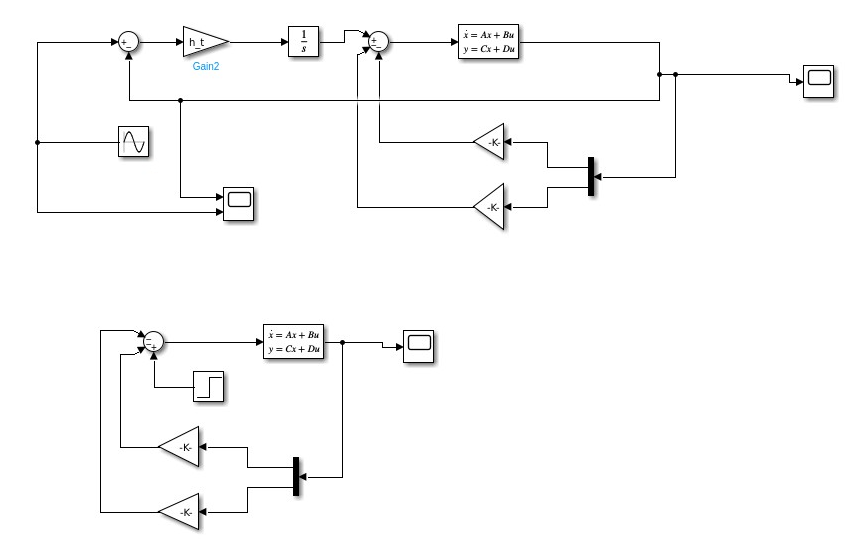
\includegraphics[width=0.75\linewidth]{simus.png}
    \caption{Diagrama no Simulink}
    \label{fig:enter-label}
\end{figure}
\section{Conclusão} 
Todo o processo de modelagem do sistema de controle em espaço de estados apresentou resultados esperados. Contudo, a modelagem por regulação mostrou-se inviável devido ao erro significativo em regime permanente na resposta ao degrau. Já o controlador por rastreio mostrou-se ideal, oferecendo uma resposta rápida e precisa tanto para uma entrada degrau quanto para outros tipos de entrada.

\end{document}



